
\chapter{Case Study}

The town of Jokela in Finland was chosen as the study study area. Pipe Network and flow meter data was provided by Tuusula Water Utility \textit{Tuusulan Vesihuolto}. The following sections provide an summary of characteristics of the catchment, data providers and data treatment, and parameter estimation for physically based and unit hydrograph methods.

\section{Jokela Town}

- where it is (also center point)
- mostly flat
- land use (just percentage)
- soil type (just percentage)
- climate (maybe mention mean temperature of months) of the last 10 years
- mean slope of each

\section{Data and Parameter Estimation}

tell about all parameters estimated for SWMM physically based model and the parameters estimated for RTK-Unit Hydrograph. Similar list with previous added comparison of PB and RTK but instead of the modules, the actual parameters and paint the most sensitive ones. 

Explain that the preliminar sensitivity analysis of parameters will be explained in this chapter. 

%===============================================================
% Sanitary Sewer Inflow and Groundwater data 
%===============================================================

    \subsection{Sanitary Sewer Flow and Groundwater Measurement Data} \label{flowdata}
    
    
    \subsection{Separation of Flow Components}

•	SSOAP toolbox allows the users to visually adjust RTK parameters comparing the flow measured values and the RTK hydrograph through an iterative process \cite{Vallabhaneni2007}. Using such tool make the process easier for modelers. However, even with such tools, manual calibration can be time consuming. This can limit the frequency that calibrations are done. Optimization algorithm is applied as an attempt to mimic this iterative process done manually by modelers.

SSOAP Toolbox developed by \ac{EPA} has tools to support the quantification and management of RDII in sanitary sewer networks. The RDII Analysis Tool available in the SSOAP Toolbox can identify and separate DWF and WWF, determine parameters for the set of Unit Hydrographs RTK, and perform statistical analysis of the parameters to non-measured catchments and design storms (Vallabhaneni and Burgess 2007). The SSOAP was used in this study to quantify RDII, other two relevant features for the choice were: 1. free and open source; 2. Interface with SWMM 5.


\begin{figure}[ht]
    \centering
	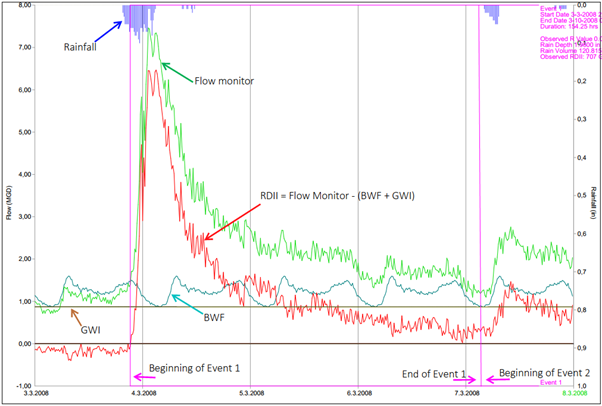
\includegraphics[scale=1.2]{figures/SSOAP_example.png}
	\caption{Graphical visualization of sanitary sewer flow components using SSOAP Toolbox}
	\label{fig:SSOAPexample}
\end{figure}

Dry Weather Flow Statistics for Meter Flow_Jokela_Smoothed

Flows are in LPS

           Average Maximum   Average   Average Minimum
Weekday       17.5046       11.3026        4.9083
Weekend       18.0745       12.5058        5.5565



average Minimum night flow

1   15.8.2018   3.0556 LPS
2   11.8.2018   3.0556 LPS
3   12.8.2018   3.2639 LPS
4   18.8.2018   3.3333 LPS
5   8.9.2018   3.3333 LPS
6   7.8.2018   3.3333 LPS
7   20.8.2018   3.4028 LPS
8   17.8.2018   3.4028 LPS
9   9.9.2018   3.5417 LPS
10   8.8.2018   3.6111 LPS



\begin{figure}[ht]
    \centering
	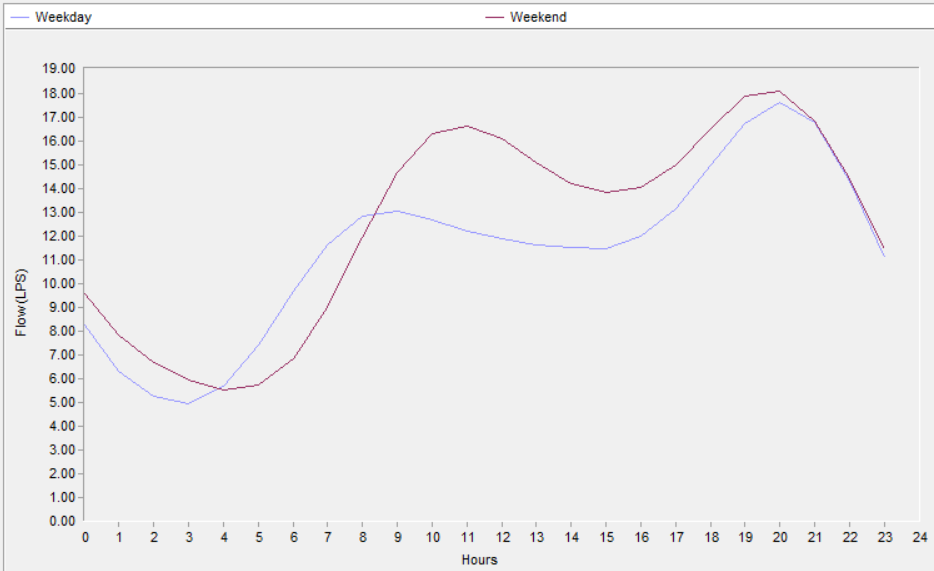
\includegraphics[scale=0.6]{figures/ssoap_dry_hydrograph.png}
	\caption{Estimated Dry-weather Hydrograph from EPA SSOAP tool}
	\label{fig:ssoapdryh}
\end{figure}
    
    
WET WEATHER determ
- minimum peak I/I LPS 0 
- minimum event duration 6h
- minimum rainfall volume mm 15


9 events defined

Event #        Start Date           End Date
--------------------------------------------
1          1.1.2018 0.00    1.21.2018 22.00
2        1.21.2018 23.00    2.18.2018 22.00
3         4.9.2018 20.00     5.26.2018 3.00
4        6.21.2018 21.00    6.22.2018 16.00
5          7.3.2018 0.00     7.4.2018 18.00
6         7.4.2018 19.00     7.7.2018 10.00
7        8.20.2018 18.00    8.21.2018 14.00
8        9.11.2018 18.00     9.14.2018 0.00
9         9.15.2018 8.00    9.19.2018 23.00



\begin{figure}[ht]
    \centering
	\includegraphics[scale=1.2]{figures/ssoap_wet_hydrograph.png}
	\caption{Estimated Wet-weather Hydrograph from EPA SSOAP tool}
	\label{fig:ssoapweth}
\end{figure}    

- holidays in Finland were not counted (total of 15 days)
- dry days with no rainfall with a period of X
- Current, previous and two days previous maximum allowed rainfall amount set to zero. From three to seven previous days maximum rainfall set to 10mm.
Determining Weekday Statistics...
 Number of days written = 78
 Number of days lost    = 286
                      AVERAGE (LPS)   STANDARD DEVIATION (LPS)
Average Daily Flow      12.3646                  4.1401
Maximum Daily Flow      18.6477                  5.3117
Minimum Daily Flow      6.0559                  3.9778

Eliminating Weekdays...
 Number of days written = 66
 Number of days lost    = 298
                      AVERAGE (LPS)   STANDARD DEVIATION (LPS)
Average Daily Flow      11.3778                  1.7468
Maximum Daily Flow      17.6507                  2.4096
Minimum Daily Flow      4.9255                  1.5036


Determining Weekend Statistics...
 Number of days written = 36
 Number of days lost    = 328
                      AVERAGE (LPS)   STANDARD DEVIATION (LPS)
Average Daily Flow      14.3232                  6.2980
Maximum Daily Flow      20.5264                  7.9425
Minimum Daily Flow      7.0682                  5.5326

Eliminating Weekend days...
 Number of days written = 32
 Number of days lost    = 332
                      AVERAGE (LPS)   STANDARD DEVIATION (LPS)
Average Daily Flow      12.5058                  2.3451
Maximum Daily Flow      18.3138                  2.9730
Minimum Daily Flow      5.4570                  2.2070


- \& of GWI assumed
-there were X available days after excluding the above mentioned. The mean flow for each hour of these days was defined as the DWF.


Include Table here with "water balance" 
- Month - Peak Flow [l/s] - Mean flow [l/s] - NRW [m³] - \% of GWI


Before smoothing
Maximum Flow = 90.600 LPS @ 5.7.2018 1.00.00
Minimum Flow = 0.300 LPS @ 4.6.2018 12.00.00
Average Flow = 15.104 LPS

after smoothing
Maximum Flow = 81.573 LPS @ 5.1.2018 10.00.00
Minimum Flow = 1.701 LPS @ 12.8.2018 4.00.00
Average Flow = 15.104 LPS
%===============================================================
% Meteorological data
%===============================================================


    \subsection{Meteorological Data} \label{meteodata}
    meteorological data is presented for both historical and forecast. 
    TELL HERE GENERAL THINGS ABOUT THE DATA THAT ARE EQUAL TO ALL SUBSUBSECTIONS I.E. THE PROVIDER, FORECAST MODEL, ETC.
        \subsubsection{Precipitation}
        Give characteristics of the data here, graphics and etc
        \subsubsection{Temperature}
        Give characteristics of the data here, graphics and etc
        One missing data that was filled using linear interpolation between the previous and next hour.
        \subsubsection{Wind}
        Give characteristics of the data here, graphics and etc

%===============================================================
% Snow data and param estimation
%===============================================================

\subsubsection{Snow Depth}

\begin{figure}[h]
    \centering
	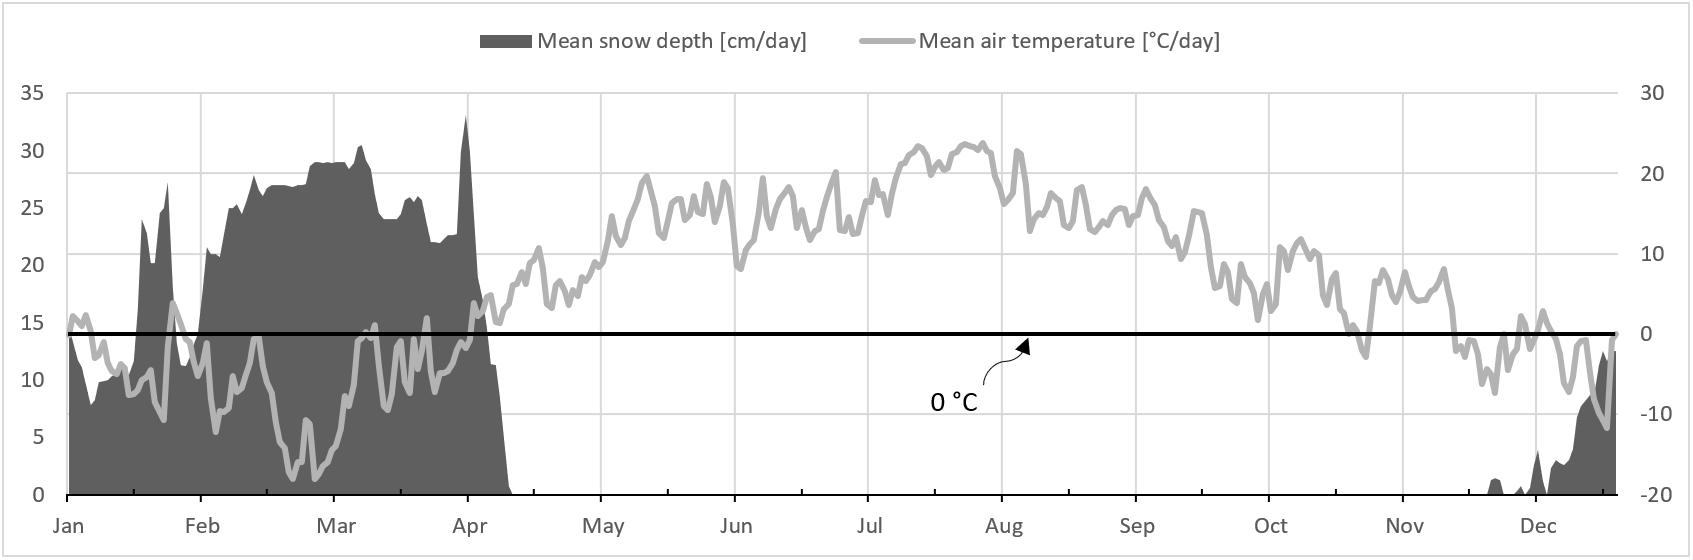
\includegraphics[scale=0.45]{figures/measuredsnowpack.png}
	\caption{Snow depth and Temperature Measurements \citet{fmidata}}
	\label{fig:snowmeasurement}
\end{figure}
        
Estimation of parameters was carried based on the range proposed in section \ref{snowlit}. Sensitivity analysis was carried by manually varying individual parameters while others were static. It was found that the degree-hour melt coefficients ($DHM_{min}$, $DHM_{max}$), dividing temperature ($SNOTMP$), base temperature ($T_{base}$) and snow catch factor ($SCF$).

Base temperature and dividing temperature were initially estimated by observing relations among hourly temperature and snow depth. Whenever the snow depth measurement varied, values of temperature where collected. Temperatures during the increase of the snow depth were stored to estimate the dividing temperature($SNOTMP$) whereas temperatures during decrease of snow depth were used to estimate the base temperature($T_{base}$). Periods when the temperatures were out of the range limited (see table \ref{tbl:snowparam}) were discarded. The mean of the stored temperature were then used as the final estimation of $SNOTMP$ and $T_{base}$ and were respectively  0.1°C and -1.9°C. It is important to emphasize that this was a rough estimate used only to input initial values for the simulations. $DHM_{min}$ and $DHM_{max}$ were set initially as the limits of table \ref{tbl:snowparam}. $TIPM$ and $RNM$ were set as used by \citet{Rossman2016} and \citet{anderson1973}. No information on the rain gauge deficiency to record snowfall and fraction of free water capacity values were assessed. Therefore, $SCF$ and $FWFRAC$ values were set initially to their middle range. Two parameters for initial condition of the simulation are also required: 1. Initial depth of water equivalent ($SD_0$); 2. initial free water ($FW_0$). The first was estimated as 10\% of the first measured value of snow depth assuming a ratio of 10:1 for the snow pack depth and water equivalent depth as rule of thumb suggested by \citet{Rossman2016}.
    
Figure \ref{fig:snow1sim} show the results of the simulation using the initially estimated parameters and the results of a simulation with parameters manually calibrated. Four first months of 2018 between 1\textsuperscript{st} of January and 15\textsuperscript{th} of April when all the snow depth measured was already melted.

\begin{figure}[h]
    \centering
	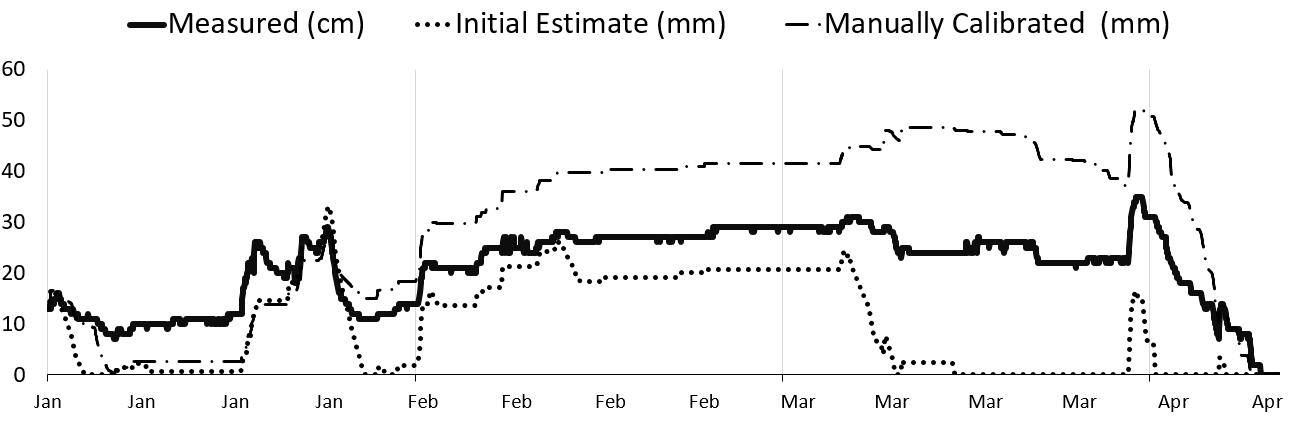
\includegraphics[scale=0.55]{figures/snowdepth_1st_simulations.png}
	\caption{Results of Initial parameter estimation x manual calibration of Snowpack \& Snowmelt parameters}
	\label{fig:snow1sim}
\end{figure}
    
By a visual analysis of the results of the first simulation and comparison to the measured snow depth values, it is possible to identify a higher rate of melt and snow accumulation than the values measured. This was corrected after a manual calibration of parameters. A lower rate of snow accumulation was achieved by assuming that the rain gauge was able better measure the snowfall. Therefore, $SCF$ was reduced to 1.2. To reduce melting rate, the temperature which snow melt starts ($T_{base}$) was increased to its upper limit of 0°C. Although the results were better, a higher melt rate than expected was still with the pack being completely melted around three weeks before the expected time. Therefore, the minimum melt coefficient ($DHM_{min}$) was lowered further than its lower range limit from 0.019[mm/°C-h] to 0.001[mm/°C-h].

%SCF, among the sensitive parameters, were calibrated aiming to find a smaller range of sensitive parameters to describe the study area reducing the amount of possible values. 

Table \ref{tbl:snowparamest} depicts the initially estimated parameters, parameter values after manual calibration against measured data, and changes in the previously proposed range based on literature review (see table \ref{tbl:snowparam}) after results of the manual calibration. The only changed was a reduction of $DHM_{min}$ parameter of approximated 47\%. 

\begin{table}[h]
\caption{Snowpack \& Snowmelt estimated parameters \cite{Rossman2016}}
\label{tbl:snowparamest}
\centering
\begin{tabular}{lcccc}
\toprule
\textbf{Parameter} & \textbf{\begin{tabular}[c]{@{}c@{}}Initially\\ Estimated\end{tabular}} & \textbf{\begin{tabular}[c]{@{}c@{}}Manually\\ Calibrated\end{tabular}} & \textbf{\begin{tabular}[c]{@{}c@{}}Changes in \\ Previous Range\end{tabular}} & \textbf{Calibrated} \\ \hline
SNOTMP             & 0.1                                                                                        & 0.1                                                                                        & -                                                                                                 & {[}°C{]}            \\
SCF                & 1.5                                                                                        & 1.2                                                                                        & -                                                                                                 & {[}1{]}             \\
T\textsubscript{b}                 & - 1.9                                                                                      & 0                                                                                          & -                                                                                                 & {[}°C{]}            \\
DHM\textsubscript{min} - DHM\textsubscript{max}          & 0.019 - 0.10                                                                               & 0.009-0.03                                                                                 & 0.009 - 0.15                                                                                      & {[}mm/°C-h{]}       \\
RNM                & 0.6                                                                                        & 0.6                                                                                        & -                                                                                                 & {[}1{]}             \\
FWFRAC             & 0.13                                                                                       & 0.13                                                                                       & -                                                                                                 & {[}1{]}             \\
TIPM               & 0.5                                                                                        & 0.5                                                                                        & -                                                                                                 & {[}1{]}             \\
SD\textsubscript{0}                & 13                                                                                         & 13                                                                                         & -                                                                                                 & {[}mm{]}            \\
FW\textsubscript{0}                & 0                                                                                          & 0                                                                                          & -                                                                                                 & {[}mm{]}           
\end{tabular}
\end{table}

%===============================================================
% Topographic data
%===============================================================
        
    \subsection{Topographic Data}
    DEM
    LAND USE
    http://metatieto.ymparisto.fi:8080/geoportal/catalog/search/resource/details.page?uuid=%7B26EEEBBB-FB5C-4045-B6DF-439F9B7D5C46%7D
    
    example of table for mannings 
    file:///C:/Users/PedroAlmeida/Documents/Thesis/References/An_Operational_Method_for_Flood_Directive_Implementation.pdf
    
    URBAN AREA
    IMPERVIOUSNESS
    \subsubsection{Soil Superficial Deposits}
    
    The soil type coverage data was fetched from \acf{GTK} \cite{gtkdata} through its open data online service and was used to estimate the three parameters of Horton infiltration (see, \ref{infiltration}). The available information was obtained as vector data containing superficial deposits of Finland with material produced between 1972-2007. GIS operations were carried using Qgis to delimit the area concerned Jokela's catchment. Coverage of superficial deposit is depicted in figure \ref{fig:supdeposits}. Mixed soil types were simplified to facilitate model's parameter estimations.\\
    
\begin{figure}[h]
    \centering
	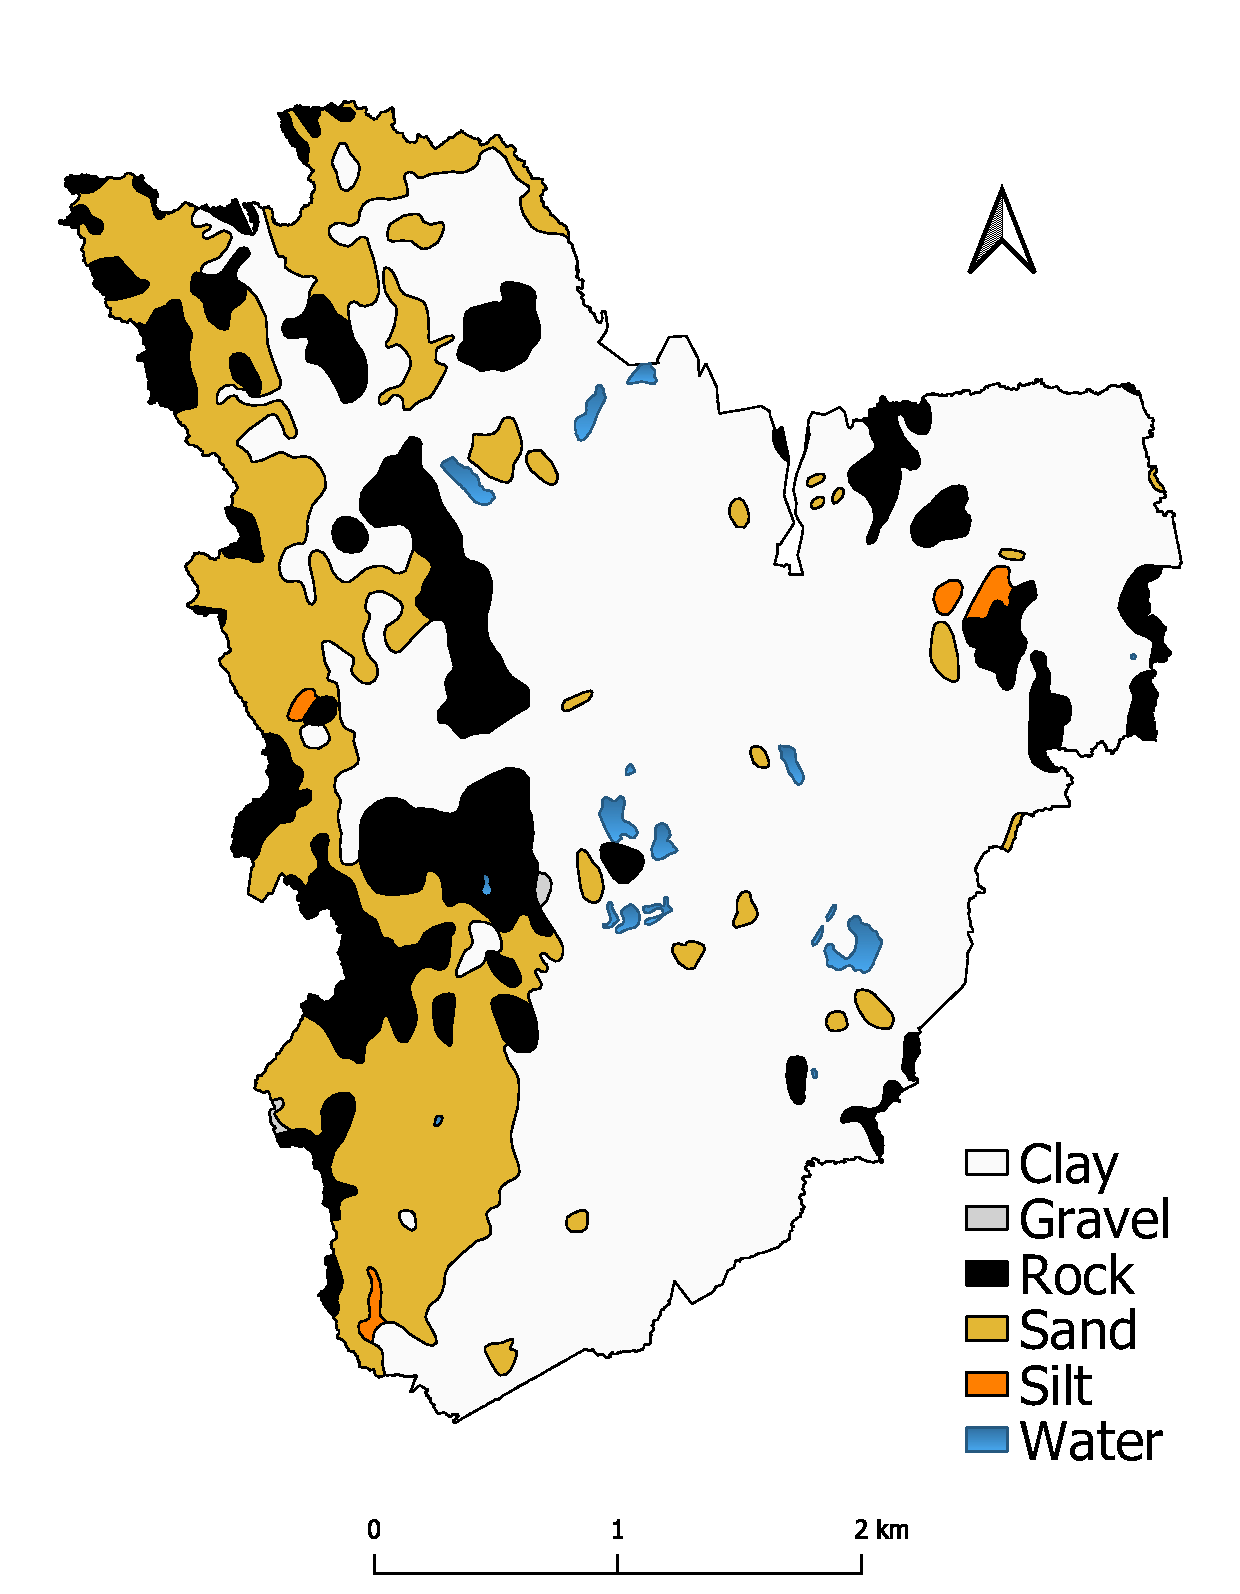
\includegraphics[scale=0.4]{figures/Jokela_Superficial_Deposits.pdf}
	\caption{Jokela catchment soil superficial deposits}
	\label{fig:supdeposits}
\end{figure}

As informed in section \ref{infiltration}, there are four parameters necessary to satisfy the Modified Horton infiltration model: Initial infiltration capacity ($f_0$); Minimum infiltration capacity ($f_\infty$), decay coefficient ($k_d$), and recovery coefficient ($k_r$) that is calculated based on drying time. For simplicity, the parameters were averaged by the whole area of Jokela catchment without considering subcatchment's divisions per pumping station. Therefore, it is assumed that all subcatchments have the same parameters for the infiltration model. Estimation of parameters was carried as follows:
\begin{enumerate}
    \item Initial infiltration capacity ($f_0$): values per soil type as estimated by \citet{Rossman2016} for DRY soils multiplied by 1.2 to account for vegetation present in the catchment.
    \item Minimum infiltration capacity ($f_\infty$): considered equal to saturated hydraulic conductivity with values estimated by \citet{Rawls1983} and available in SWMM user help.
    \item Decay coefficient ($k_d$): set to 4 [h\textsuperscript{-1}] as suggested by \citet{Rossman2016}.
    \item Recovery coefficient ($k_r$) in days: equation \ref{eqn:k_r} as function of minimum infiltration capacity in inches/hour.
\end{enumerate}

\begin{equation}
\label{eqn:k_r}
k_r = \frac{3.125}{\sqrt{f_\infty}}
\end{equation}


The estimation of each parameter for each soil type is depicted in table \ref{tbl:infparamest}. Area and percentage of coverage for each soil type was also calculated to spatially weight $f_0$, $f_\infty$, and $k_r$ using equation \ref{eqn:infilaverage} to obtain a unique value of each parameter to represent the entire catchment.


\begin{table}[h]
\caption{Modified Horton infiltration parameter estimation}
\label{tbl:infparamest}
\centering
\begin{tabular}{@{}lccccc@{}}
\toprule
\textbf{soil type} & \textbf{area [ha]} & \textbf{coverage [\%]} & \textbf{$f_0$} & \textbf{$f_\infty$} & \textbf{$k_r$} \\
\midrule
Clay               & 887.5                 & 66.0                       & 30.5          & 0.3                            & 28.8          \\
Sand               & 267.9                 & 19.9                       & 152.4         & 117.8                          & 1.5           \\
Rock               & 181.6                 & 13.5                       & 3.0           & 0.03                            & 90.9          \\
Silt               & 5.9                   & 0.4                        & 91.4          & 6.5                            & 6.2           \\
Gravel             & 1.2                   & 0.1                        & 1524.0        & 1180.0                         & 0.5           \\
Water              & 11.5                  & 0.9                        & -             & -                              & -             \\ \midrule
Total              & 1355.7                & 100.0                      & -             & -                              & - \\           
\bottomrule
\end{tabular}
\end{table}

\begin{equation}
\label{eqn:infilaverage}
Parameter = \sum_{n}^{m}(Parameter_n \cdot Coverage_n \cdot 0.1)
\end{equation}
where: \\
\indent $parameter$ = $f_0$, $f_\infty$ or $k_r$ \\
\indent $n$ = soil type (excluding water) \\

after applying equation \ref{eqn:infilaverage} was applied to the estimated parameters of table \ref{tbl:infparamest}. The result of $k_r$ was set to its upper limit range since it was greater than 14 days because of the predominance of soil types with relatively low saturated hydraulic conductivity (\textit{Clay and Rock}). The following unique parameters were obtained and included to SWMM model:

\begin{center}
  $f_0$ = 52.2 [mm/h], $f_\infty$ = 24.6 [mm/h], $k_d$ = 4 [1/h], $k_r$ = 14 [days]  
\end{center}





%===============================================================
% Groundwater case study
%===============================================================
\subsection{Groundwater} \label{gwcs}

As mentioned in the literature ((Bennett et al. 1999; Vallabhaneni and Burgess 2007), (Barden et al. 2011), and others), infiltration into the sewer lines can be caused by the seasonal elevation of groundwater table or other condition that increased soil moisture content causing a temporary saturated zone. Elevation of the groundwater table around Jokela town was assessed in this section as an attempt to identify a possible correlation with seasonal variations of the water table and the flow measurements of the town’s sanitary sewer network. 
Information of water table levels was provided by the Finnish Environmental Institute (SYKE) through its open data service (“Finnish Environment Institute (SYKE) Open Environmental Information Systems” n.d.). Data of three observation wells were available surrounding Jokela town as depicted in Figure 4. The recording period and routines among the three stations varies considerably - from one record per month to one record per year.

Picture

Measurements from 2004 to 2016 from station 0118651 -located southeast from Jokela- were combined and plotted in Figure 5. Years with less than six months recorded were left out: 2007; 2008; and 2017. All the eleven years records showed an elevation on the groundwater table from March to May. 

Picture

Only yearly measurements were available for the closest station 0154356 located around 5km west from Jokela. The records are from different months, mostly during spring and summer. Therefore, assessment of monthly variation for the same year was not possible. However, the available data suggests slightly higher water table levels on average from January to June for the period of 1999-2017.

Picture

The closest observation well with data available from 2018 was 110651. Measurements from 2018 were relevant to compare with flow measurements of the same year in the sewer network. As depicted in Figure 6, the groundwater elevation period is on average from February to May. Similar pattern as observed for station 0118651. For 2018, periods of February-March and April-May were presented elevation in the groundwater table. If a similar groundwater elevation pattern also occurred for Jokela town in 2018, located 9 km away, correlation between aquifer recharge periods and higher infiltration rates into the sanitary sewer exists. 
    
    
    \subsection{Weather Forecast}

\section{Data Treatment}

\section{Snowmelt and Rainfall for calibration and validation}



remind: Importance to use radar data and refer the literature vallabhnai conclusions of using radar and pawel nawalani that compared radar x rain gauge. 

remind: put a graph of variations in precipitation and temperature to justify that more data should be assessed. 


\section{Jokela Sanitary Sewer Model}

    \subsection{Hydraulic Model}
    
    \subsection{Physically-Based: SWMM Modules}


        \subsubsection{Jokela Sewershed Delineation}

\texttt{\textit{Area}} is one of the parameters necessary for many SWMM modules as described in equations X, XXU,XX,XX, and table x x X of previous sections. The definition of the \texttt{\textit{Area}} parameter for \acf{SSN} is rather conceptually challenging since it is located under the surface. This is due the different components of \ac{WWF}: surface/direct flow or sub-surface/infiltration flow gradient and the area of influence of each of these two processes. Rain drop falling over a specific point on the surface. The drop can flow over the surface towards the direction of the steeper slope or infiltrate and then flow through the porous in the soil to a very different direction than . As 
Therefore, delineating the sewershed only the \acf{DEM} rainfall-runoff

The sewershed delineation is a discretization of the space domain. The area division that supplies water to to a specific point within the \ac{SSN}. When modeling natural rivers, this area is assumed as all regions where a rain drop would flow downstream following the soil surface slopes from high elevations towards the lowest parts due to gravitational force. This method, however, is not conceptually valid for \ac{SSN} once the network's slopes are not always as the terrain slopes. Therefore, \ac{SSN} has a different gradient than the surface in some parts and pumping stations are required to transport waste water towards the \acf{WWTP}. This is the reason why the space domain was discretized per pimping station in this study.


Two reasons:
- Terrain slope
- Available historical flow measurements.

Qgis application was chosen to perform GIS operations and delineate sewersheds due to its free open services. GRASS r.watershed. 


Pumping stations are usually located in areas with lower surface elevation when compared to its upstream pipe network to direct the flow utilizing gravitational force and reduce energy consumption. However, differences between soil surface and network still exists in some parts of the pumping station upstream service area. 


\begin{figure}[h]
    \centering
	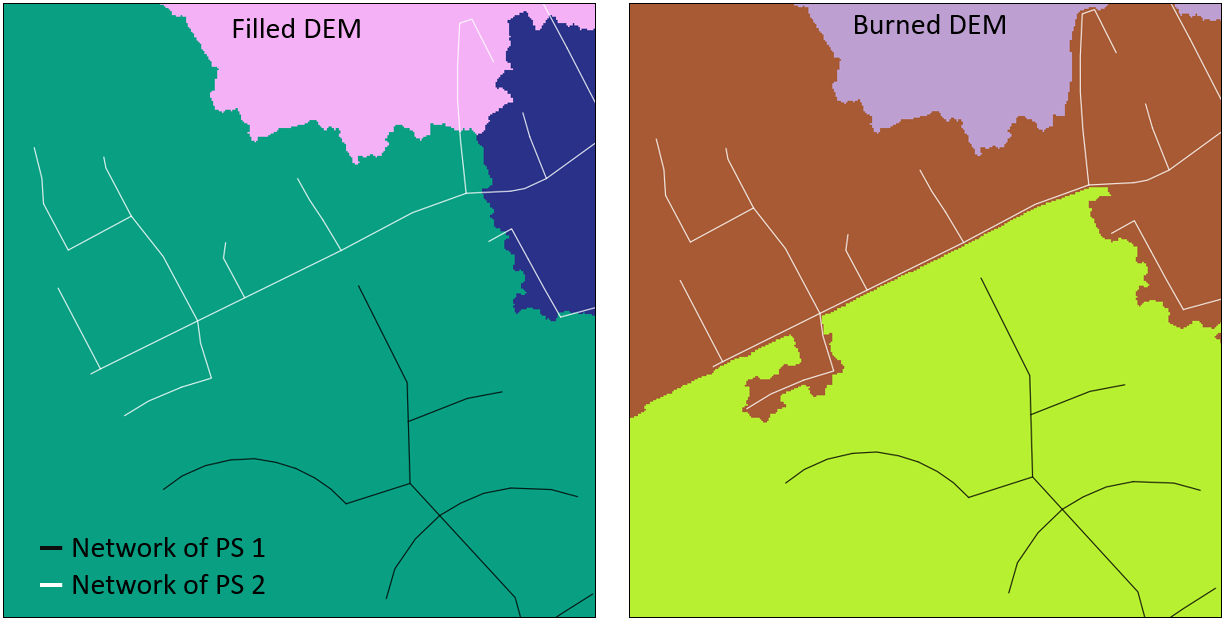
\includegraphics[scale=0.6]{figures/burnedxfilledDEM.png}
	\caption{Comparison of sewershed delineation using Filled and Burned DEM}
	\label{fig:filledxburned}
\end{figure}


, not all parts of.
The discretization in this study was DEM  Service area cadastral parcels.

Tell other options based on the network age, size, estimated defects, material, etc. 


Groundwater
         
DEM One of the first steps to model SWMMre are many ways to delineate a sewershed. The threshold level of discretization of the space domain. Each pipe section can have its own subcatchment 
          
          
         \textit{GRASS - v.clean} to split where streams intersect.
         \textit{QGIS - Merge Lines} To merge streams within the same layer. 
         \textit{QGIS - Split with lines} to split the sewershed polygon where the stream crosses.
        
        
        \subsubsection{Parameter Estimation}
    
    range of parameters are presented in each subsection of \ref{hydraulicmodel} chapter. 
    
    table \ref has the choice of parameters for all modules. The column \textit{Source} shows the references used to estimate the parameter as well as description of the data in previous section \ref{data}.
    
    Table
    
    \subsection{Synthetic Unit Hydrograph: RTK}
        
        \subsubsection{Parameter Estimation}



%===============================================================
% SIMULATIONS
%===============================================================

\section{Simulations}


